\chapter{Diseño e Implementación} % Main chapter title

\label{Chapter3} % Change X to a consecutive number; for referencing this chapter elsewhere, use \ref{ChapterX}
\definecolor{mygreen}{rgb}{0,0.6,0}
\definecolor{mygray}{rgb}{0.5,0.5,0.5}
\definecolor{mymauve}{rgb}{0.58,0,0.82}

\lstset{ %
  backgroundcolor=\color{white},   % choose the background color; you must add \usepackage{color} or \usepackage{xcolor}
  basicstyle=\footnotesize,        % the size of the fonts that are used for the code
  breakatwhitespace=false,         % sets if automatic breaks should only happen at whitespace
  breaklines=true,                 % sets automatic line breaking
  captionpos=b,                    % sets the caption-position to bottom
  commentstyle=\color{mygreen},    % comment style
  deletekeywords={...},            % if you want to delete keywords from the given language
  %escapeinside={\%*}{*)},          % if you want to add LaTeX within your code
  %extendedchars=true,              % lets you use non-ASCII characters; for 8-bits encodings only, does not work with UTF-8
  %frame=single,	                   % adds a frame around the code
  keepspaces=true,                 % keeps spaces in text, useful for keeping indentation of code (possibly needs columns=flexible)
  keywordstyle=\color{blue},       % keyword style
  language=[ANSI]C,					% the language of the code
  %otherkeywords={*,...},           % if you want to add more keywords to the set
  numbers=left,                    % where to put the line-numbers; possible values are (none, left, right)
  numbersep=5pt,                   % how far the line-numbers are from the code
  numberstyle=\tiny\color{mygray}, % the style that is used for the line-numbers
  rulecolor=\color{black},         % if not set, the frame-color may be changed on line-breaks within not-black text (e.g. comments (green here))
  showspaces=false,                % show spaces everywhere adding particular underscores; it overrides 'showstringspaces'
  showstringspaces=false,          % underline spaces within strings only
  showtabs=false,                  % show tabs within strings adding particular underscores
  stepnumber=1,                    % the step between two line-numbers. If it's 1, each line will be numbered
  stringstyle=\color{mymauve},     % string literal style
  tabsize=2,	                   % sets default tabsize to 2 spaces
  title=\lstname,                   % show the filename of files included with \lstinputlisting; also try caption instead of title
  morecomment=[s]{/*}{*/}%
}


%----------------------------------------------------------------------------------------
%	SECTION 1
%----------------------------------------------------------------------------------------
\section{Diseño}

En esta sección se tratan las consideraciones de diseño que se utilizaron para desarrollar el sistema siguiendo los lineamientos de trabajo planteados en la asignatura “Ingeniería de Software en Sistemas Embebidos”.  Se tomó como guía el \textit{port} de LPCOPEN v2.16 \citep{lpcopen}, provisto por NXP para la familia de microcontroladores LPC43XX, que contiene un ejemplo de aplicación sencillo que integra \mbox{freeRTOS} y lwIP.  Para el servidor web se utilizó un ejemplo de los desarrolladores del stack TCP/IP lwIP \citep{contrib}. A su vez, también fueron consultados otros ejemplos de utilización de lwIP con la CIAA \citep{ws-ridolfi} y \citep{ciaaFirmware}.

\subsection{Principio de funcionamiento}

En términos generales, un servidor web es un programa que permite publicar información en la \textit{World Wide Web} (WWW) o una red de área local (LAN). Esta información puede ser consultada desde cualquier navegador web estándar como Mozilla Firefox, Internet Explorer o Google Chrome, entre otros. El servidor opera utilizando el protocolo HTML \citep{rfc7540} en la capa de aplicación del modelo OSI \citep{OSI} y establece un canal de comunicación entre un servidor y un cliente. El servidor ejecuta las peticiones del cliente. 

En el presente trabajo, el servidor web se encuentra embebido en la plataforma CIAA y proporciona al usuario una interfaz para monitorear y controlar el sistema. El servidor web es capaz de soportar los siguientes servicios:

\begin{itemize}
\item HTTP 2.0: HyperText Transfer Protocol (HTTP) es un protocolo orientado a transacciones y sigue el esquema petición/respuesta entre un cliente y un servidor \citep{rfc7540}. En particular, la version 2.0 posibilita la utilización de conexiones persistentes o \textit{keep-alive {sessions}} que permiten transmitir múltiples pares de petición/respuesta multiplexados sobre una única conexión TCP. De esta manera se puede reducir el tráfico y mejorar el desempeño en cuanto al tiempo de respuesta del servidor web. Resulta necesario para implementar métodos AJAX.

\item SSI: \textit{Server Side Include} (SSI) es un lenguaje interpretado sencillo que consiste en un conjunto de directivas que se incluyen dentro de la codificación de una página HTML y que se evalúan en el servidor web cuando la página HTML es solicitada.  Permite incluir contenido generado en forma dinámica en tiempo de ejecución.

\item AJAX: \textit{Asynchonous JavaScript And XML} (AJAX) es un conjunto de técnicas utilizadas desde el lado del cliente para enviar y recibir información de un servidor en forma asincrónica.  Es una forma de desacoplar el intercambio de información y la visualización de la página web.  Permite que se cambie el contenido de una página web en forma dinámica sin necesidad de recargar la totalidad de la página. Para implementar AJAX, el servidor debe soportar directivas SSI.  El cliente debe soportar JavaScript para peticionar información en segundo plano y es responsable de realizar dichas peticiones a intervalos regulares.

\item Formularios web (peticiones GET): Los formularios se utilizan para enviar información al servidor.  GET es un método del protocolo HTTP que se utiliza para solicitar información de un servidor \citep{rfc2616}. Durante una petición GET se produce un \textit{request} HTTP por parte del cliente y un \textit{response} del servidor. La solicitud de información se transmite a través de la \textit{Uniform Resource Identifier} (URI) agregando parámetros a la \textit{Uniform Resource Locator} (URL).  En la presente implementación el método GET se utiliza para enviar información al servidor en lugar de utilizar lo que sería más correcto, el método POST, debido a la mayor sencillez del primero por sobre el segundo.

\item CGI (peticiones GET): \textit{Common Gateway Interface} (CGI) es un estándar que provee una interfaz sencilla para ejecutar programas externos en un servidor HTTP \citep{rfc3875}. En esta implementación se utiliza CGI para ejecutar rutinas específicas dentro del microcontrolador y generar una nueva página web como respuesta.  Las funciones asociadas a un CGI se ejecutan cuando se envía un formulario web con el método GET al servidor para su procesamiento.
\end{itemize}

%-----------------------------------
%	SUBSECTION 1
%-----------------------------------
\subsection{Arquitectura}
El sistema está diseñado con una arquitectura de capas, según se puede observar en la figura \ref{fig:bloques}.  Agrupados por color se pueden apreciar los distintos niveles de abstracción y, dentro de cada capa, los bloques funcionales que la integran .  %Esta organización permite un mayor reutilización del código

\begin{figure}[htb!]
	\centering
    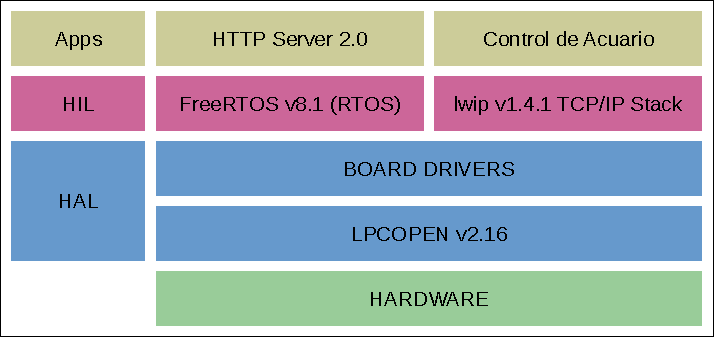
\includegraphics[width=\textwidth]{./Figures/bloques.pdf}
	\caption{Diagrama en bloques del \textit{firmware}.}
	\label{fig:bloques}
\end{figure}
	
En cuanto a los niveles de abstracción, la primer capa la constituye el \mbox{\textit{hardware}} de la plataforma CIAA. La segunda capa, \textit{Hardware Abstraction Layer} (HAL), permite desacoplar las capas superiores del \textit{hardware}. Aquí se encuentran los \textit{drivers} del fabricante del microcontrolador, en el bloque funcional LPCOPEN, y los desarrollados para la plataforma CIAA en el bloque BOARD. La capa \textit{Hardware \mbox{Independent} Layer} (HIL) incluye los módulos del RTOS y el \textit{stack} TCP/IP y, como su nombre lo indica, no está asociada a ningún \textit{hardware} en particular.  Finalmente, la última capa contiene dos aplicaciones, el servidor web y el control del acuario.



%-----------------------------------
%	SUBSECTION 2
%-----------------------------------
%\clearpage
%\subsection{Arquitectura Jerárquica}

Se puede apreciar la estructura jerárquica de archivos del sistema en la figura \ref{fig:estructura}, donde se han incluido los archivos fuente relevantes de cada bloque.

\begin{figure}[htp]
	\centering
    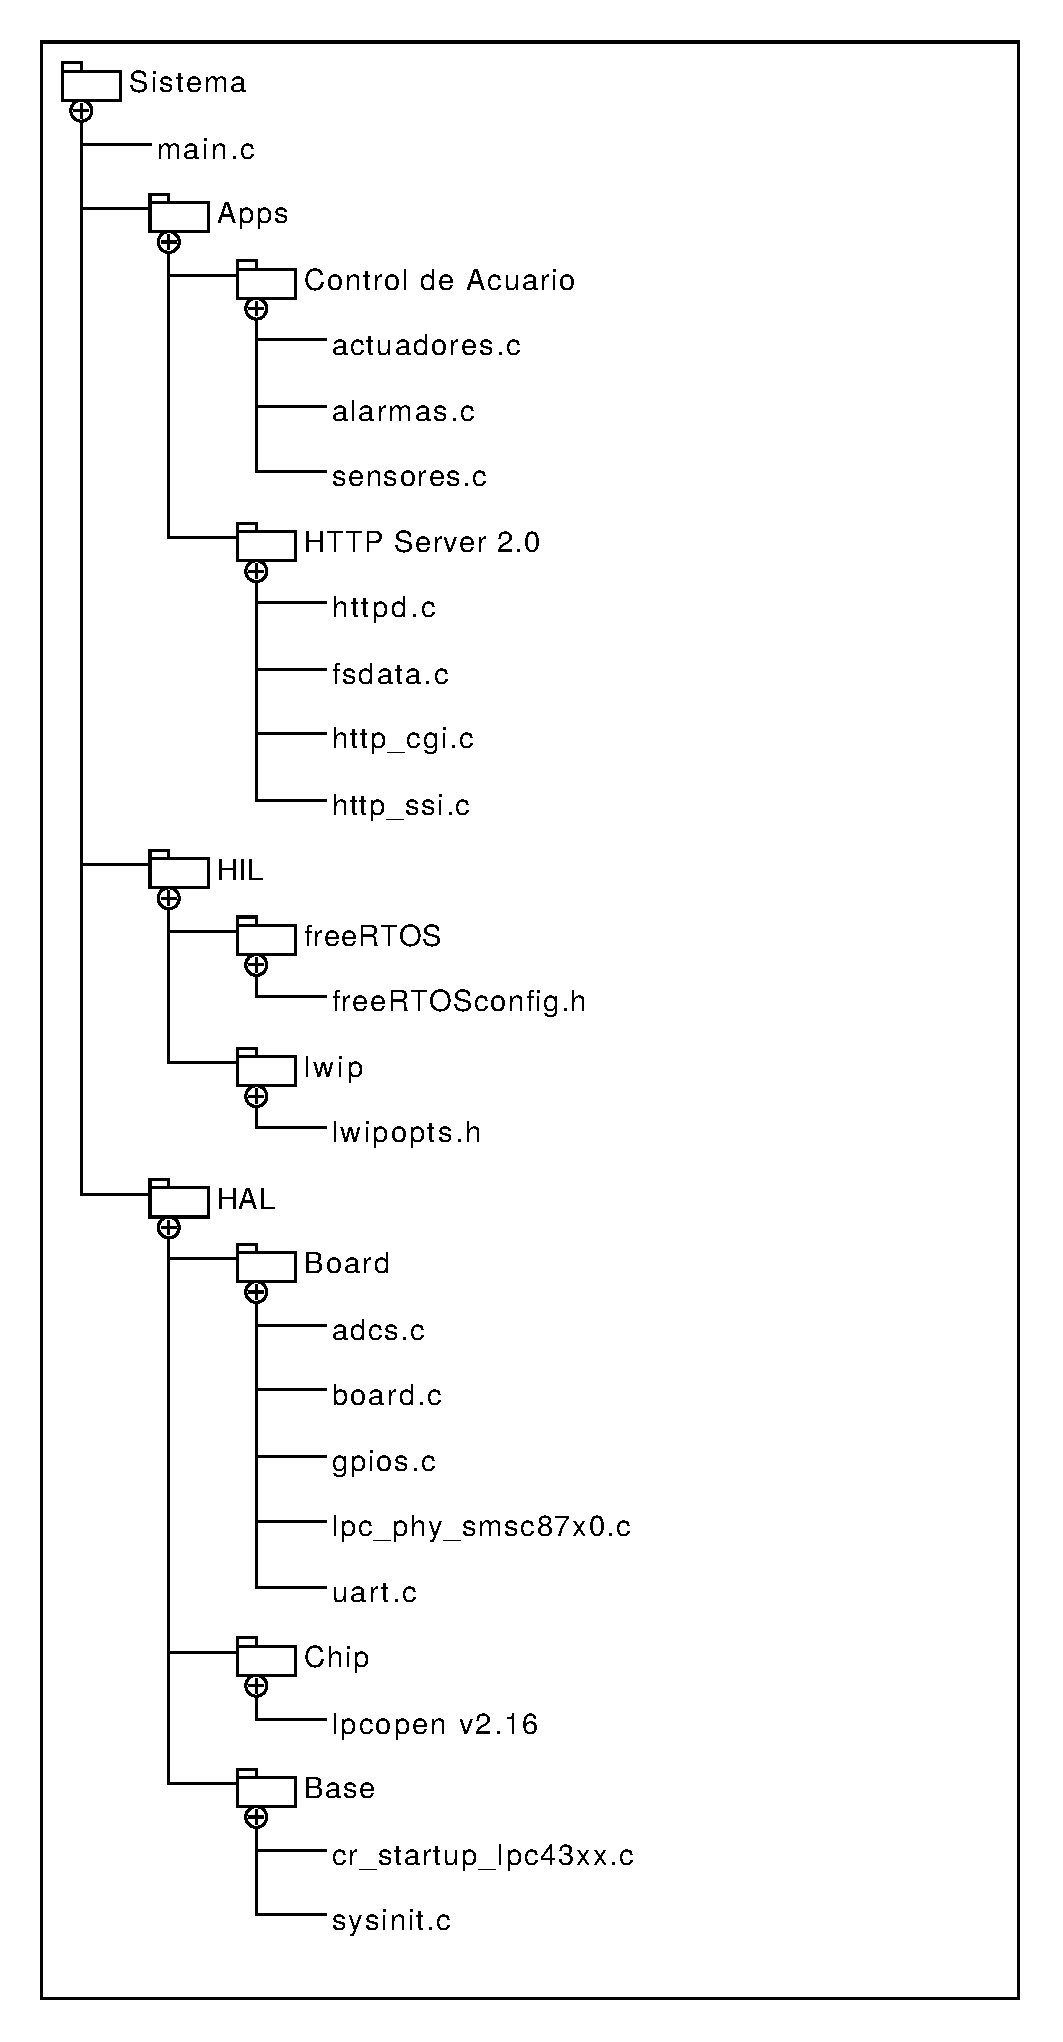
\includegraphics[width=.68\textwidth]{./Figures/diagramaUML.pdf}
	\caption{Estructura jerárquica de archivos.}
	\label{fig:estructura}
\end{figure}

\subsection{Lógica de control}

Se presenta una descripción en pseudocódigo de las funciones más relevantes de la lógica de control.  El lazo principal de control consiste en una tarea de freeRTOS, llamada vControl, que se ejecuta periódicamente a intervalos regulares de 500 ms.  Esta tarea llama secuencialmente a tres funciones auxiliares para actualizar los valores de los sensores, actualizar los valores de las alarmas y controlar los actuadores del sistema, respectivamente.

\vspace{20px}
\begin{lstlisting}[caption=Pseudocódigo del lazo principal de control.]  % Start your code-block

#define MAX_SENSOR_NUMBER 3
#define MAX_ALARM_NUMBER  6
#define MAX_ACTUATOR_NUMBER 6

uint32_t sensorValue[MAX_SENSOR_NUMBER];		
FunctionalState alarmControl[MAX_ALARM_NUMBER];	//ENABLE or DISABLE
state_t alarmState[MAX_ALARM_NUMBER];						//ON or OFF
state_t actuatorState[MAX_ACTUATOR_NUMBER];			//ON or OFF

void vControl() {

	initGlobalVariables();
	
	period = 500 ms;
		
	while(1) {

		ticks = xTaskGetTickCount();
		
		updateSensors();
		
		updateAlarms();
		
		controlActuators();
		
		vTaskDelayUntil(&ticks, period);
	}
}
\end{lstlisting}

\vspace{20px}
\begin{lstlisting}[caption=Pseudocódigo del control de los sensores.]  % Start your code-block

void updateSensors() {

	// for every sensor
	for (i=0; i < MAX_SENSOR_NUMBER; i++) {

		// read ADCs
		data_i = readDataFromADC(sensorChannel_i);

		// apply scale convertion 
		data_i = scaleConvertion(data_i, i );
	
		// impact sensor value to global variable 
		sensorValue[i] = data_i
	}
}
\end{lstlisting}

\vspace{20px}
\begin{lstlisting}[caption=Pseudocódigo del control de las alarmas.]  % Start your code-block

void updateAlarms() {

	// for every sensor; i goes from 0 to 2
	for ( i=0; i < MAX_SENSOR_NUMBER; i++ ) {
		
		//check sensor upper threshold
		if ( sensorValue[i] > sensorMaxLimit[i] ) {
			setAlarmState(2*i);	// alarmState's index goes from 0 to 5
		}
		else {
			clearAlarmState(2*i);
		}

		//check sensor lower threshold
		if ( sensorValue[i] < sensorMinLimit[i] ) {
			setAlarmState( (2*i)+1 );
		}
		else {
			clearAlarmState( (2*i)+1 );
		}
	}
}
\end{lstlisting}

\vspace{10px}
\begin{lstlisting}[caption=Pseudocódigo del control de los actuadores.]  % Start your code-block

void controlActuators() {

	state_t actuatorFakeState[MAX_ACTUATOR_NUMBER];
	
	// for every actuator, 
	for( i=0; i < MAX_ACTUATOR_NUMBER; i++ ) {
		// Get current state
		actuatorFakeState[i] = getActuatorState(i);
		
		// If control is enable checks alarm and operates actuators x,y,...
		if (ENABLE == alarmControl[i]){
		
			if( ON == alarmState[i] ) {
				actuatorFakeState[x] = (Necesary action); // ON or OFF
				actuatorFakeState[y] = (Necesary action);
				alarmFlag[i] = ON;		// flag indicates control actions underway
			}
			// alarm = OFF & flag = ON then control actions should be stoped
			else if ( ON == alarmFlag[i] ) {
				actuatorFakeState[x] = !(Necesary action);
				actuatorFakeState[y] = !(Necesary action);
				alarmFlag[i] = OFF;
			}			
		}
	}
	
	// Impact changes to actuators
	for( i=0; i < MAX_ACTUATOR_NUMBER; i++ ) {

		actuatorState[i] = actuatorFakeState[i];
	}	
}
\end{lstlisting}

%----------------------------------------------------------------------------------------
%	SECTION 2
%----------------------------------------------------------------------------------------
\clearpage
\section{Implementación}

Para acceder a los \textit{sockets}, el servidor web utiliza la RAW API\footnote{\url{http://lwip.wikia.com/wiki/Raw/TCP}} de lwIP que emplea una serie de \textit{callbacks} para manejar los eventos de la comunicación.  La función httpd\_init() inicia el demonio del servidor y debe ser llamada luego de que el stack se encuentre inicializado con la función lwip\_init().  Para alojar el contenido HTML que se debe servir se utiliza un sistema de archivos dedicado implementado en ROM \citep{webserver}. A través del \textit{script} makefsdata, provisto por lwIP, se puede personalizar los archivos HTML e integrarlos al sistema mediante el archivo fuente fsdata.c.  Se debe tener especial cuidado al utilizar las funciones de la RAW API en un entorno con múltiples hilos de ejecución como freeRTOS, ya que las funciones no cuentan con protección frente a accesos concurrentes.  Las funciones de esta API deben ser invocadas desde un único hilo de ejecución.


 
%Passive connection (Listen)
%
%    Call tcp\_new to create a pcb.\\
%    Optionally call tcp\_arg to associate an application-specific value with the pcb.\\
%    Call tcp\_bind to specify the local IP address and port.\\
%    Call tcp\_listen or tcp\_listen\_with\_backlog. (note: these functions will free the pcb given as an argument and return a smaller listener pcb (e.g. tpcb = tcp\_listen(tpcb)))\\
%    Call tcp\_accept to specify the function to be called when a new connection arrives. Note that there is no possibility of a socket being accepted before specifying the callback, because this is all run on the tcpip\_thread.\\

El servidor inicia con la configuración detallada en la tabla \ref{tab:config}.

\begin{table}[ht]
	\centering
	\caption{Configuración MAC del servidor web.}
	\begin{tabular}{@{} l l  @{}}    \toprule
		\emph{\textbf{Parámetro}} & \emph{\textbf{Valor}}  \\
		\midrule
		Dirección MAC	& 00:60:37:12:34:56 	\\
		DHCP				& Deshabilitado		\\ 		
		Dirección IP		& 192.168.200.99		\\
		Máscara de red	& 255.255.255.0		\\ 
		Puerta de enlace	& 192.168.200.1		\\ 
		Puerto			& 80					\\ 
		\bottomrule
		\hline
	\end{tabular}
	\label{tab:config}
\end{table}

%-----------------------------------
%	SUBSECTION 3
%-----------------------------------
\subsection{Interfaz web embebida}
\label{sec:interfaz-web}

Se presenta la interfaz web implementada para monitorear y controlar el acuario.  Esta consta de un menú de navegación en la parte izquierda, que permite acceder a tres pantallas, detalladas a continuación:

\begin{itemize}
\item Inicio, con un resumen del estado del sistema sin posibilidad de modificaciones. Se puede observar en la figura \ref{fig:interfazHome}.
\item Control, donde se encuentran los controles para operar las alarmas y actuadores. Se puede observar en la figura \ref{fig:interfazControl}.
\item Configuración, donde se puede cambiar la configuración de red del servidor. Se muestra en la figura \ref{fig:interfazConfig}. 
\end{itemize}

En la página inicio se pueden observar tres bloques de información referida a los sensores, las alarmas y los actuadores, respectivamente.  Esta información se actualiza una vez por segundo mediante el método AJAX, según está documentado en la sección \ref{sec:ajax}. El estado de las alarmas se indica como ``NORMAL'' en color verde o ``ALARMA'' en color rojo cuando el control automático está habilitado, o el mismo texto en gris cuando el control automático está deshabilitado.  El estado de los actuadores se indica como ``ENCENDIDO'' en color verde o ``APAGADO'' en color rojo sin importar el estado del control de alarmas.

\begin{figure}[htp]
	\centering
    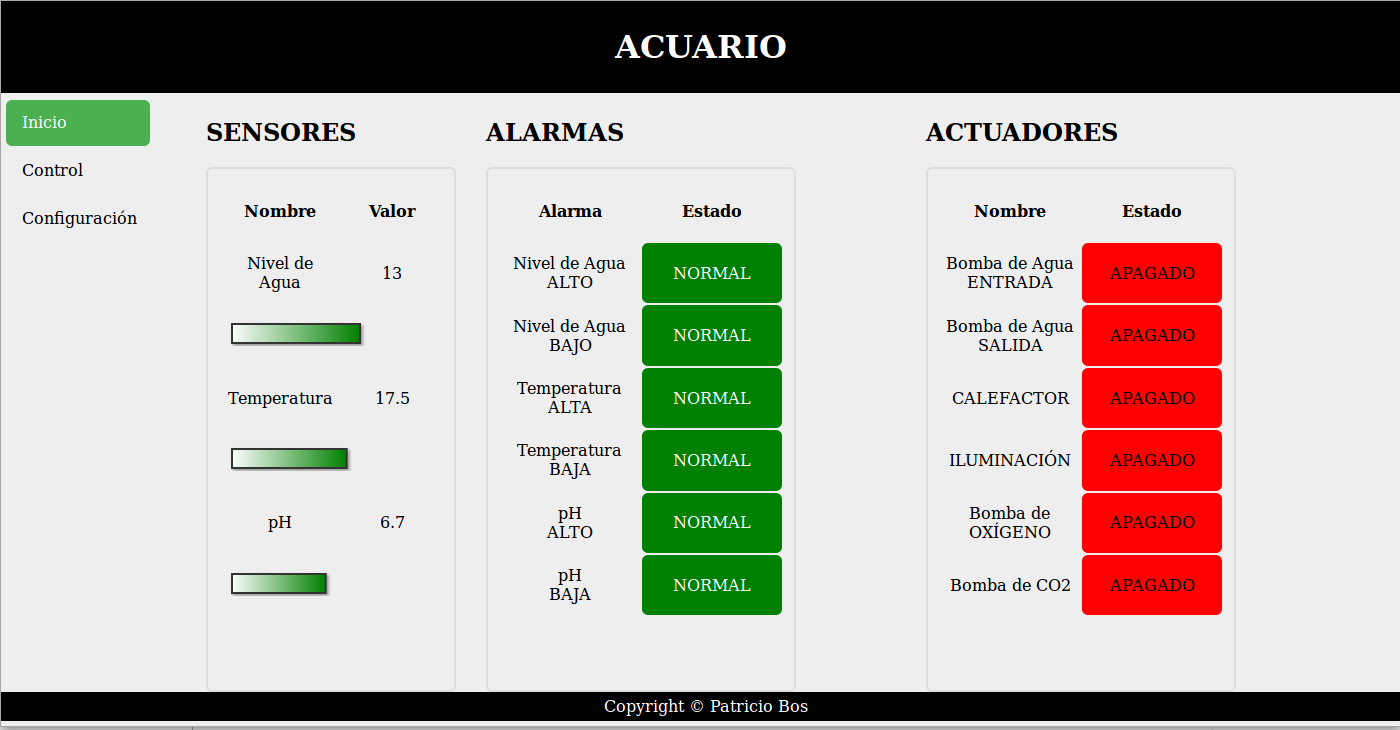
\includegraphics[width=\textwidth]{./Figures/interfaz_home_normal}
	\caption{Interfaz web: página principal Inicio.}
	\label{fig:interfazHome}
\end{figure}

\begin{figure}[htp]
	\centering
    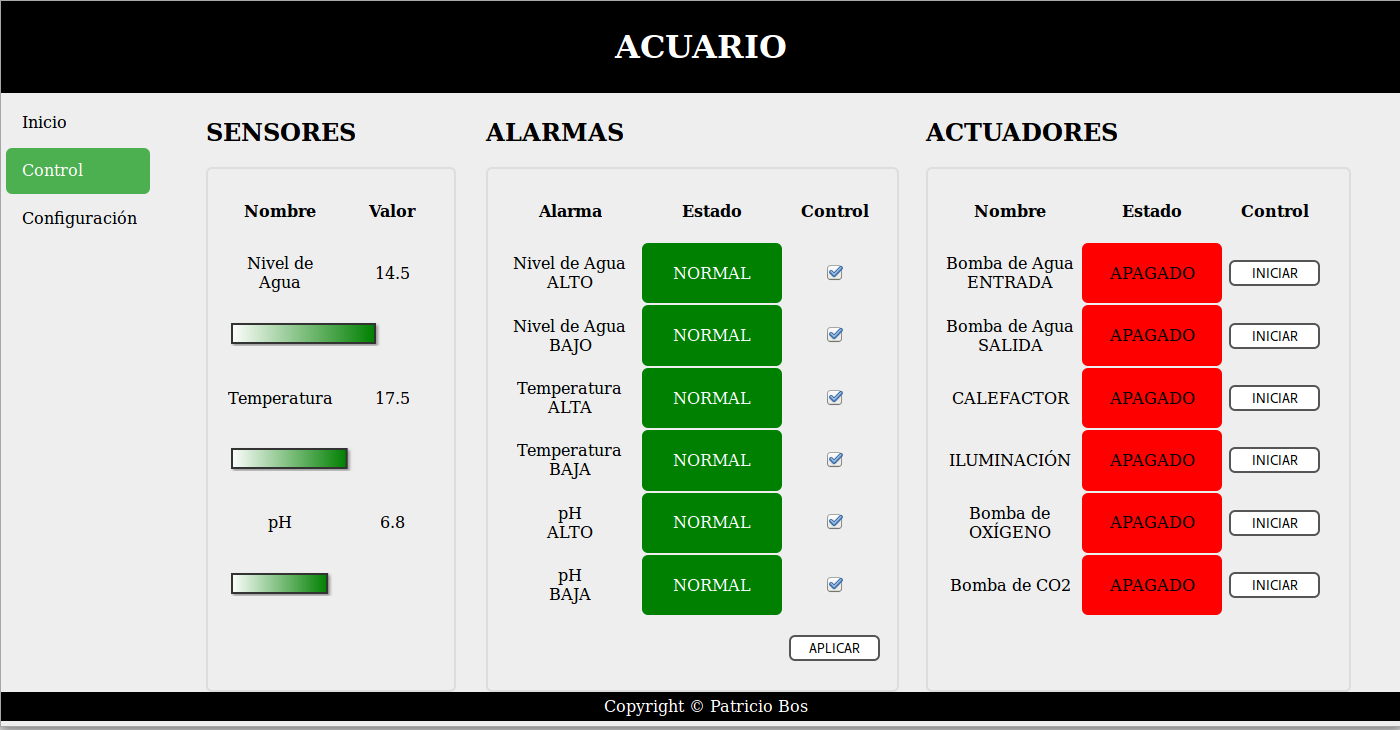
\includegraphics[width=\textwidth]{./Figures/interfaz_control_normal}
	\caption{Interfaz web: página para controlar el sistema.}
	\label{fig:interfazControl}
\end{figure}

\begin{figure}[htp]
	\centering
    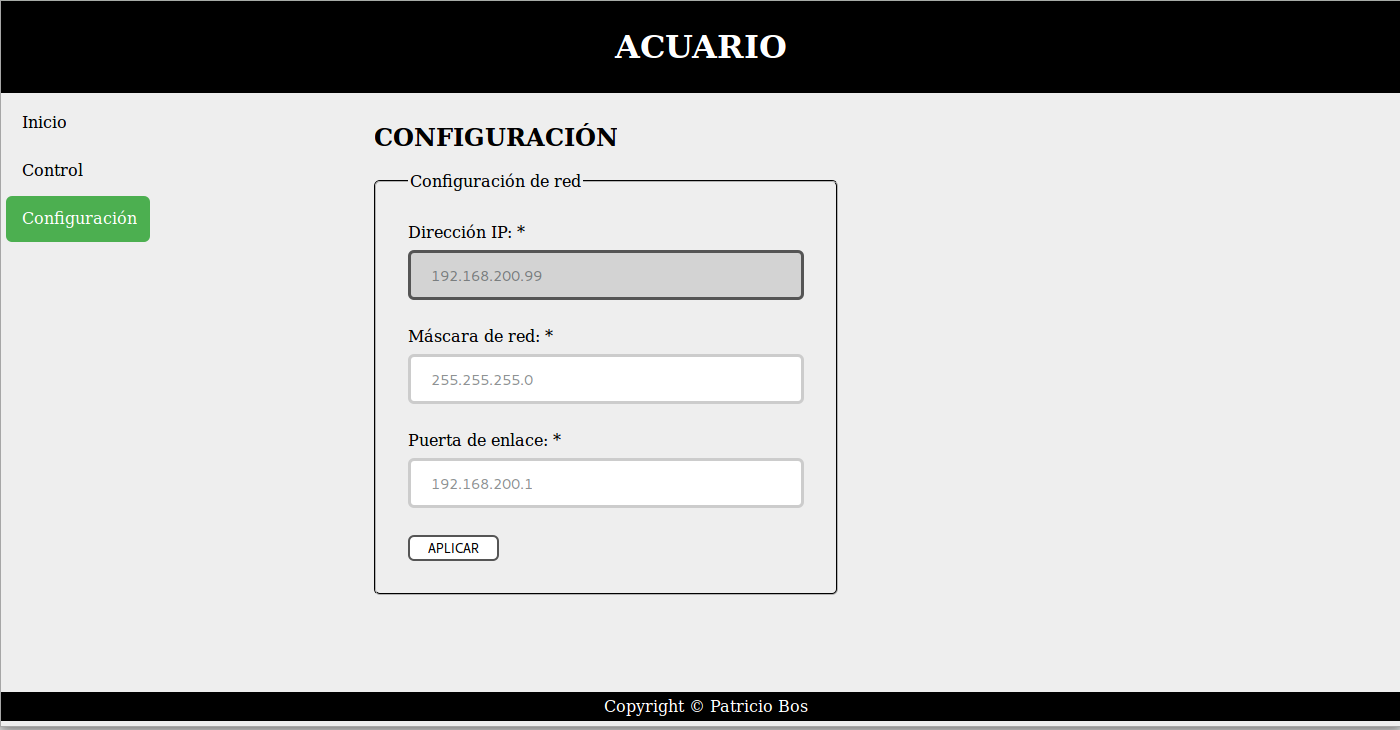
\includegraphics[width=\textwidth]{./Figures/interfaz_config}
	\caption{Interfaz web: configuración de red.}
	\label{fig:interfazConfig}
\end{figure}

Tanto en la página Inicio como en la página Control, en el apartado SENSORES se muestra el valor numérico de cada sensor junto con una representación gráfica de dicho valor.  Se utiliza un gráfico de barra horizontal proporcional al valor numérico que se construye en tiempo de ejecución mediante rutinas de JavaScript.  Cada sensor tiene una escala que se ajusta según su valor máximo definido dentro del microcontrolador.  Mientras exista una condición de alarma para un sensor, tanto por exceso como por defecto, la gráfica asociada se muestra en color rojo, caso contrario se muestra en color verde.

La página Control, según se puede observar en la figura \ref{fig:interfaz3}, posee además de la información mostrada en la página Inicio, columnas llamadas ``control'' para operar sobre las alarmas y los actuadores, respectivamente.  

En el apartado ALARMAS se encuentra un \textit{checkbox} para cada alarma que permite habilitar el control automático sobre la condición de alarma o deshabilitarlo.  Notar que existe un botón ``APLICAR'' al final de la columna de control que impacta el contenido de los \textit{checkboxes} en la lógica de control dentro del microcontrolador. Para lograr esto se utiliza el método CGI según se documenta en la sección \ref{sec:cgi}.  El valor seleccionado/no seleccionado de los \textit{checkboxes} se guarda en los datos de sesión del navegador web del cliente.

\vspace{30px}


\begin{figure}[hp]
	\centering
    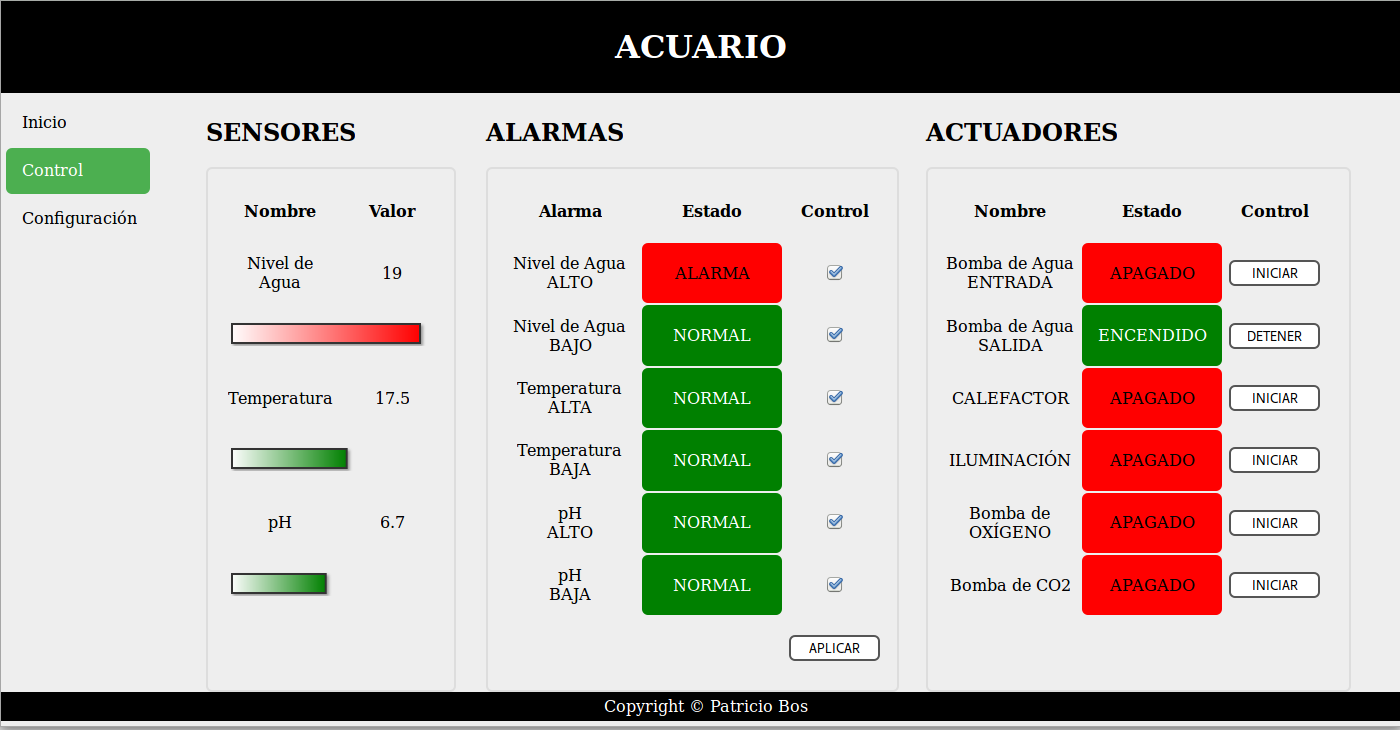
\includegraphics[width=\textwidth]{./Figures/interfaz_control_alarma1}
	\caption{Interfaz web: condición de alarma presente.}	
	\label{fig:interfaz3}
\end{figure}

\vspace{35px}

En el apartado actuadores, y dentro de la columna control, se pueden observar botones para iniciar o detener los actuadores en forma manual.  En el caso particular que se muestra en la figura \ref{fig:interfaz3}, frente a la condición de alarma por nivel de agua alto, la lógica de control mantiene la bomba de entrada apagada y la bomba de salida encendida.  Los botones de los actuadores mencionados se encuentran deshabilitados mientras la alarma esté presente y si fueran presionados no producirían efectos sobre el sistema.  Al posar el cursor sobre un botón deshabilitado aparece un cuadro de diálogo como se muestra en la figura \ref{fig:interfaz4}, indicando que se debe deshabilitar el control de alarma para operar el actuador manualmente.



\begin{figure}[ht!]
	\centering
    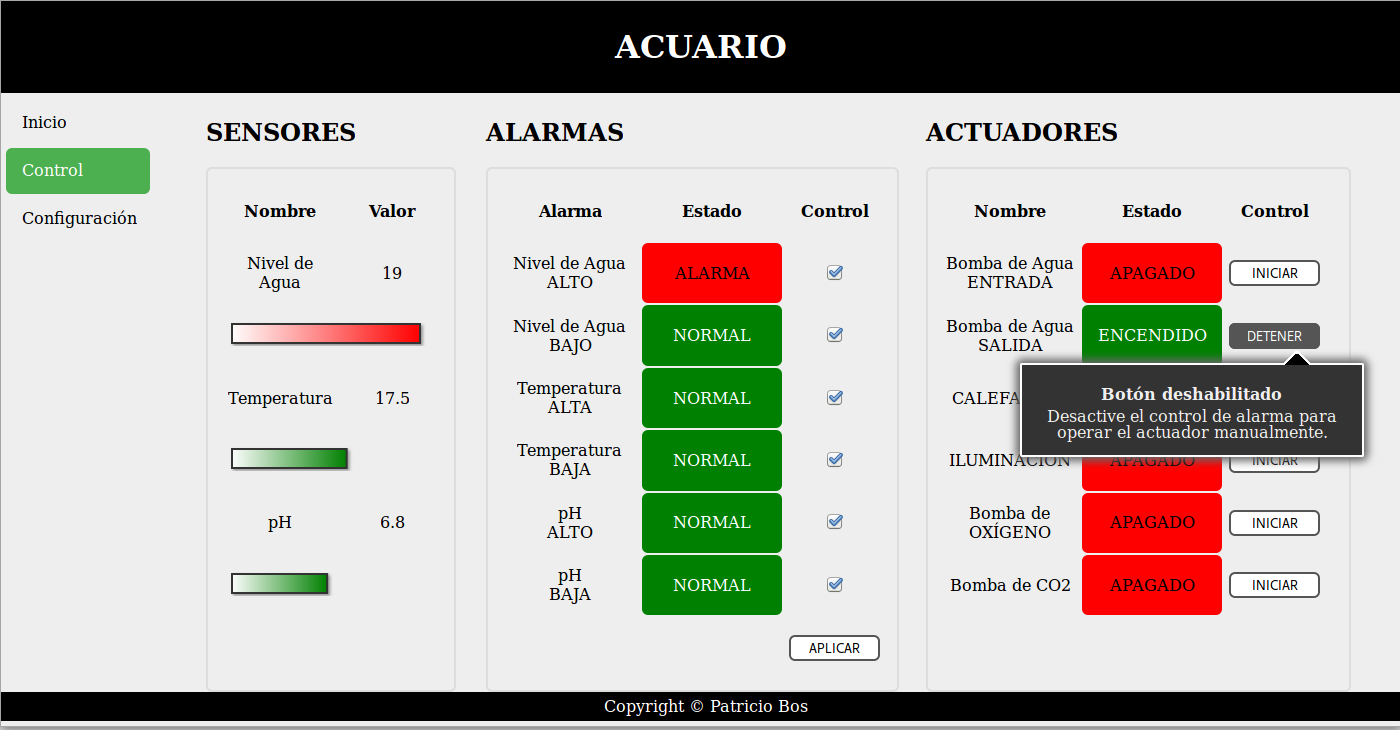
\includegraphics[width=1\textwidth]{./Figures/interfaz_control_alarma2}
	\caption{Interfaz web: botón deshabilitado por el control.}
	\label{fig:interfaz4}
\end{figure}

\vspace{35px}

Cuando el control automático de una alarma se encuentra deshabilitado, el texto ``NORMAL'' o ``ALARMA'' se muestra sobre un fondo gris, como se puede observar en la figura \ref{fig:interfaz5}. Como ya fuera mencionado, los actuadores asociados a esta condición son las dos bombas de agua que para el caso del control automático deshabilitado no se encuentran inhibidos y pueden ser operados manualmente.  Cabe mencionar que en la figura \ref{fig:interfaz5} se puede ver cómo la bomba de agua SALIDA se encuentra apagada pese a que la condición de alarma se encuentra presente.  Sin pérdida de generalidad, este comportamiento puede extenderse para la totalidad de las condiciones de alarma y sus actuadores asociados.

\vspace{25px}

\begin{figure}[hp]
	\centering
    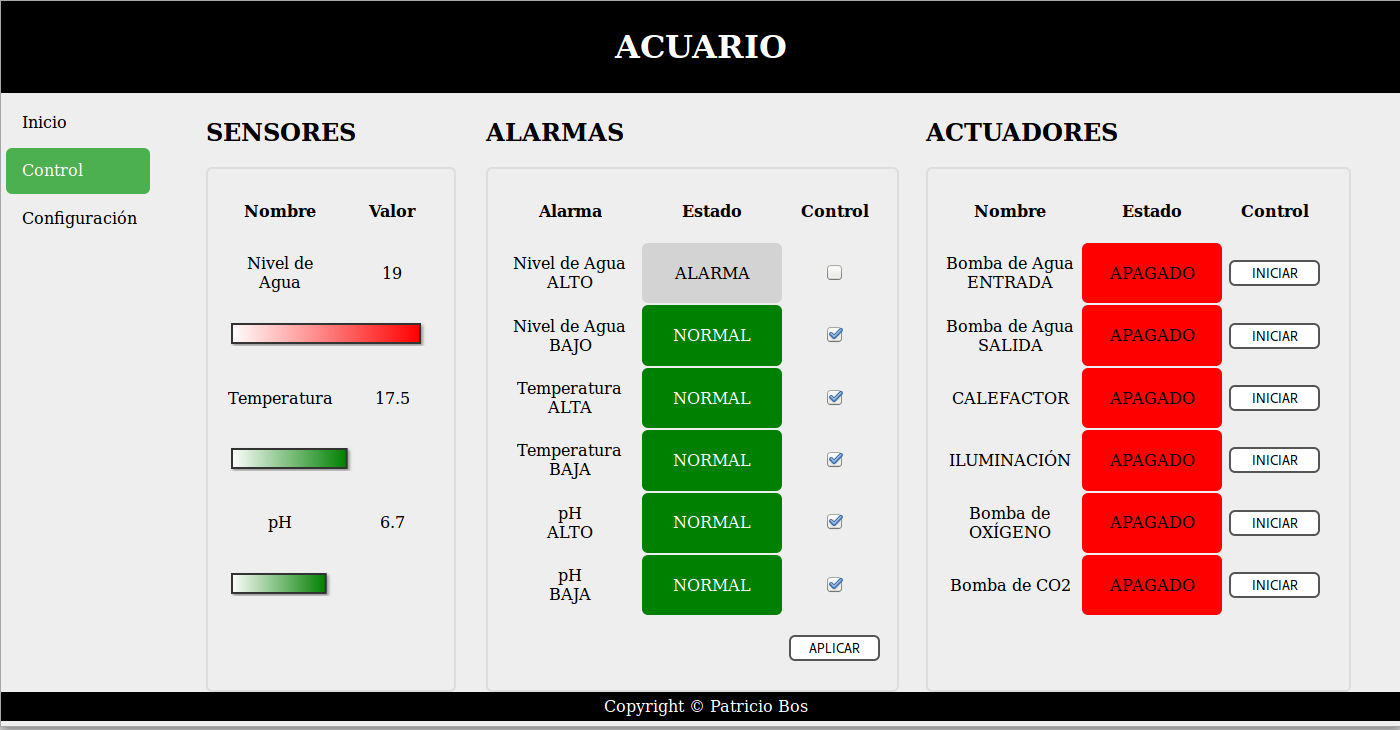
\includegraphics[width=1\textwidth]{./Figures/interfaz_control_alarma3}
	\caption{Interfaz web: control deshabilitado.}
	\label{fig:interfaz5}
\end{figure}

\clearpage
%-----------------------------------
%	SUBSECTION 4
%-----------------------------------

\subsection{Server Side Includes}
\label{sec:ssi}

La interfaz web contiene información del estado del sistema que se genera en forma dinámica en tiempo de ejecución. Mediante directivas SSI embebidas en las páginas HTML, el servidor web reemplaza cadenas de caracteres debidamente señalizadas por el contenido dinámico.  En el algoritmo \ref{alg:ssiHandler} se muestra la función que inicializa el soporte para SSI, registrando la función que se debe llamar para manejar las directiva SSI, la lista de etiquetas válidas y el número de etiquetas.

%  LWIP_DEBUGF(HTTPD_DEBUG, ("http_set_ssi_handler\n"));
%
%  LWIP_ASSERT("no ssi_handler given", ssi_handler != NULL);
%  LWIP_ASSERT("no tags given", tags != NULL);
%  LWIP_ASSERT("invalid number of tags", num_tags > 0);


\begin{lstlisting}[caption={Inicialización del SSI handler}, morecomment={[s]{/*}{*/}}, label={alg:ssiHandler}]  % Start your code-block

/** Set the SSI handler function.
  *
  * @param ssi_handler the SSI handler function
  * @param tags an array of SSI tag strings to search for in SSI-enabled files
  * @param num_tags number of tags in the 'tags' array
  */
void http_set_ssi_handler(tSSIHandler ssi_handler, const char **tags, int num_tags) {

  g_pfnSSIHandler = ssi_handler;
  g_ppcTags = tags;
  g_iNumTags = num_tags;
}
\end{lstlisting}

Se instala en manejador de directivas SSI con la siguiente línea de código:

\begin{lstlisting}
http_set_ssi_handler(SSIHandler, pccSSITags, sizeof( pccSSITags ) / sizeof( char * ) );
\end{lstlisting}

\vspace{-15px}
Las etiquetas tienen la forma de comentario HTML,	\textless ! \-- \-- \# tag \-- \-- \textgreater  donde la palabra ``tag'' se debe reemplazar por los distintos valores particulares. Se utilizaron las etiquetas definidas en el algoritmo \ref{alg:ssitag} para el estado encendido/apagado de los actuadores, los valores de los sensores, el estado normal/alarma de las alarmas y el control automático activado/desactivado, respectivamente.

\begin{lstlisting}[caption={Definición de etiquetas SSI}, label={alg:ssitag}]  % Start your code-block

// The SSI strings that are embedded in the served html files.
static const char *pccSSITags[] = {
	"act0",
	"act1",
	"act2",
	"act3",
	"act4",
	"act5",
	"sensor0",
	"sensor1",
	"sensor2",
	"alarma0",
	"alarma1",
	"alarma2",
	"alarma3",
	"alarma4",
	"alarma5",
	"ctrlAlrm0",
	"ctrlAlrm1",
	"ctrlAlrm2",
	"ctrlAlrm3",
	"ctrlAlrm4",
	"ctrlAlrm5" };
\end{lstlisting}

A continuación se presenta, en el algoritmo \ref{alg:ssihandler}, un ejemplo parcial de la función para reemplazar las etiquetas embebidas en el código HTML por el contenido dinámico.  El ejemplo se restringe por simplicidad a las primeras seis etiquetas, referidas al estado de los actuadores y puede ser extendido al resto de las etiquetas de manera análoga. 

Se muestra la función SSIHandler que es invocada cada vez que el servidor HTTPD detecta una etiqueta de la Forma \textless ! \-- \-- \# tag \-- \-- \textgreater en un archivo con extensión .shtml, .ssi o .shtm, donde ``tag'' aparece como una de las etiquetas suministradas a http\_set\_ssi\_handler en el \textit{array} ppcTags. El parámetro iIndex proporciona el índice de base cero de la etiqueta como se encuentra en el \textit{array} ppcTags e identifica la etiqueta que se va a procesar.


\begin{lstlisting}[caption={Handler de etiquetas SSI},label={alg:ssihandler}]  % Start your code-block

uint16_t SSIHandler( int iIndex, char *pcBuffer, int iBufferLength )
{

	// Unused parameter. 
	( void ) iBufferLength;

	// The SSI handler function that generates text depending on the index of the SSI tag encountered. 

	char *ptrState;

	switch( iIndex )
	{

	case ssiACT0_INDEX:
		ptrState = getActuatorCharState(portNum_0);
		strcpy( pcBuffer, ptrState );
		break;

	case ssiACT1_INDEX:
		ptrState = getActuatorCharState(portNum_1);
		strcpy( pcBuffer, ptrState );
		break;

	case ssiACT2_INDEX:
		ptrState = getActuatorCharState(portNum_2);
		strcpy( pcBuffer, ptrState );
		break;

	case ssiACT3_INDEX:
		ptrState = getActuatorCharState(portNum_3);
		strcpy( pcBuffer, ptrState );
		break;

	case ssiACT4_INDEX:
		ptrState = getActuatorCharState(portNum_4);
		strcpy( pcBuffer, ptrState );
		break;

	case ssiACT5_INDEX:
		ptrState = getActuatorCharState(portNum_5);
		strcpy( pcBuffer, ptrState );
		break;
	
	return strlen( pcBuffer );
}
\end{lstlisting}

La cadena de caracteres que se copia en pcBuffer se agrega luego de la etiqueta ``\textless ! \-- \-- \# tag \-- \-- \textgreater'' en el archivo que se envía al cliente.

%\clearpage


%-----------------------------------
%	SUBSECTION 5
%-----------------------------------
\subsection{Common Gateway Interface}
\label{sec:cgi}

Se utilizan funciones CGIs asociadas a la petición de un nombre específico de archivo.  La interfaz web, a través de un formulario GET, solicita un archivo con extensión .cgi al servidor y envía en la URL los argumentos para la función CGI. En el algoritmo \ref{alg:cgiHandler} se muestra la función para iniciar el soporte CGI que recibe como argumento un \textit{array} de pares ``nombre de archivo''/función.  Las funciones registradas se ejecutan cuando el cliente solicita el archivo con extensión .cgi asociado.  

\begin{lstlisting}[caption={Handler de funciones CGI},label={alg:cgiHandler}]  % Start your code-block

/** Set an array of CGI filenames/handler functions
  * @param cgis an array of CGI filenames/handler functions
  * @param num_handlers number of elements in the 'cgis' array
  */

void http_set_cgi_handlers(const tCGI *cgis, int num_handlers) {

  LWIP_ASSERT("no cgis given", cgis != NULL);
  LWIP_ASSERT("invalid number of handlers", num_handlers > 0);
  
  g_pCGIs = cgis;
  g_iNumCGIs = num_handlers;
}
\end{lstlisting}

Se instala en manejador de funciones CGI con la siguiente línea de código:

\begin{lstlisting}
http_set_cgi_handlers(cgi_handlers, (sizeof (cgi_handlers) / sizeof (tCGI) ) );
\end{lstlisting}

\vspace{-15px}
En el algoritmo \ref{alg:cgiHandlers} se pueden ver las definiciones de pares ``nombre de archivo''/función. Estas funciones manejan el estado encendido/apagado de los actuadores y el estado habilitado/deshabilitado del control automático de las alarmas, respectivamente.

\begin{lstlisting}[caption={Registro de nombres y funciones CGI},label={alg:cgiHandlers}]  % Start your code-block

tCGI cgi_handlers[]={

		{"/actuadores.cgi",actuatorsHandler},
		{"/alarmas.cgi",alarmsHandler}
};
tCGI * ptrCGIHandlers;
\end{lstlisting}

%-----------------------------------
%	SUBSECTION 6
%-----------------------------------
\clearpage
\subsection{AJAX}
\label{sec:ajax}

La implementación del servidor web soporta \textit{Asynchronous JavaScript and XML} (AJAX). AJAX es un método que permite actualizar el contenido de una página web en segundo plano, o sin recargar la totalidad de la página.  El navegador web es responsable de solicitar regularmente un pequeño archivo con la información que se debe actualizar y de ubicar dicha información en lugares específicos de la página web. Todas las transacciones se inician a través del navegador web del lado del cliente. La utilización de este método da un aspecto dinámico al contenido web. 

Para la utilización de AJAX se requiere que :

\begin{itemize}
\item El cliente solicite el archivo con extensión .ssi o .shtml a intervalos regulares (1 segundo) y que el servidor pueda suministrar el archivo.
\item El código fuente HTML embebido en el servidor contenga sentencias AJAX.
\item El archivo solicitado esté escrito usando directivas SSI. De esta manera, dentro del servidor se reemplazan las etiquetas SSI y la operatoria resulta transparente para el cliente.
\item El servidor web soporte la característica HTTP \textit{persistent connection} que está incluida en el \textit{stack} TCP/IP lwIP.
\end{itemize}

Se presenta en la figura \ref{fig:ajax} un diagrama de secuencia con las transacciones entre el navegador del cliente y el servidor.  Como ya fuera mencionado, el navegador es responsable de iniciar la transacción y luego procesar y posicionar la respuesta del servidor.  En el código fuente HTML embebido en el servidor se encuentran una serie de funciones en JavaScript que periódicamente realizan una petición de la página ajax.shtml, que contiene las directivas SSI, y luego procesan la respuesta.

\begin{figure}[htb!]
	\centering
    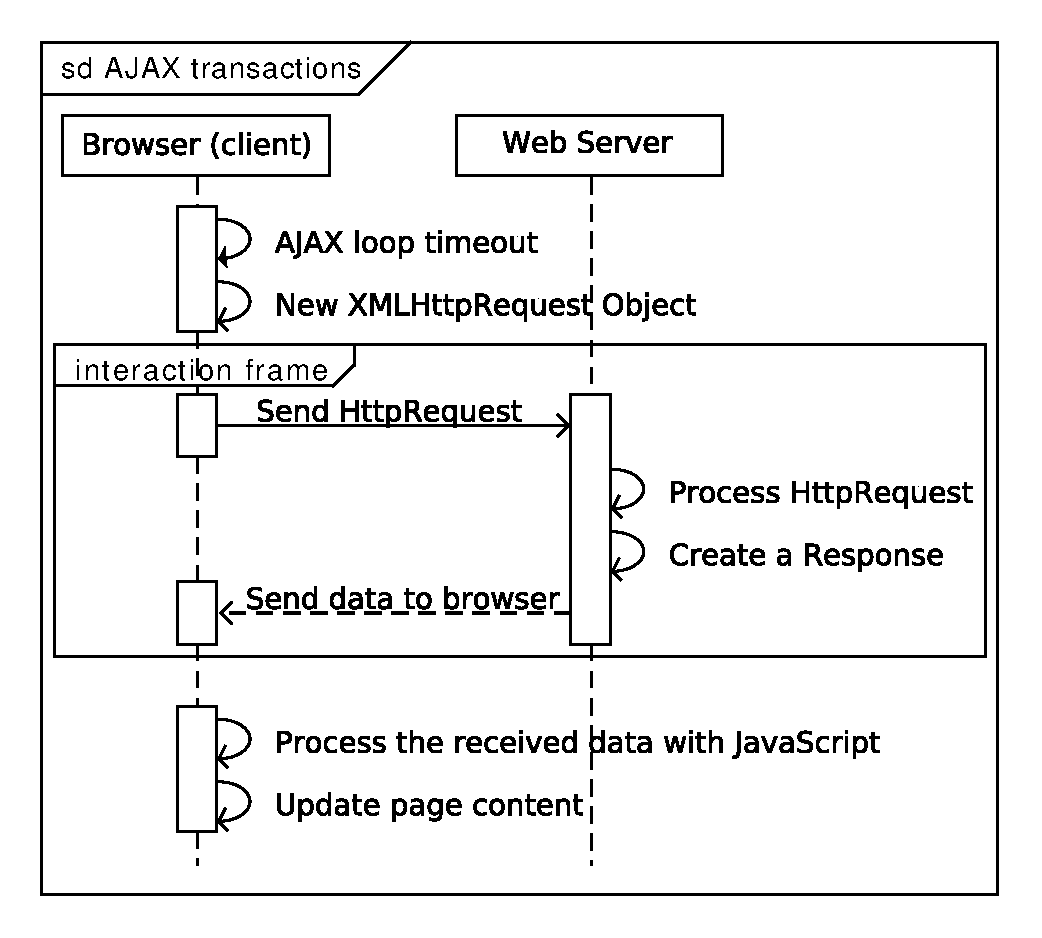
\includegraphics[width=.7\textwidth]{./Figures/ajax.pdf}
	\caption{Diagrama de secuencia AJAX.}
	\label{fig:ajax}
\end{figure}

%----------------------------------------------------------------------------------------
%	SECTION 3
%----------------------------------------------------------------------------------------

%\section{Hardware}

